\documentclass[10pt]{article}

% %%%%%%%%%%%%%%%%%%%%%%%%%%%%%%%%%%%%%%%%%%%%%%%%%%%%%%%%%%%%%%%%%%%%%%%%%%%%%%
% %                                 PACKAGES                                   %
% %%%%%%%%%%%%%%%%%%%%%%%%%%%%%%%%%%%%%%%%%%%%%%%%%%%%%%%%%%%%%%%%%%%%%%%%%%%%%%
% Identifies input coming with an UTF-8 format
\usepackage[utf8]{inputenc}
% Uses 8-bit T1 fonts (Latin) 
\usepackage{setspace}
 \singlespacing
% Arial font.
\usepackage[scaled]{helvet}
\renewcommand\familydefault{\sfdefault}
\usepackage[T1]{fontenc}
\setlength{\parindent}{0.4cm}
% Equations
\usepackage{amsmath}
% Enum Item
\usepackage{enumitem}
% Easy Lists
\usepackage[ampersand]{easylist}
% Tables
\usepackage{booktabs}
\usepackage{longtable}
% Formatting margins
\usepackage{geometry}
 \geometry{
 a4paper,
% left=25mm,
% top=25mm,
% right=25mm,
% left=25mm
 }
% Hyperreferences
\usepackage{hyperref}
% Images
\usepackage{graphicx}
% Set images location
\usepackage{wrapfig}
% Position for tables and images
\usepackage{float}
% Blibliography
\usepackage[backend=biber, style=numeric]{biblatex}
 \addbibresource{artAPA.bib}

% %%%%%%%%%%%%%%%%%%%%%%%%%%%%%%%%%%%%%%%%%%%%%%%%%%%%%%%%%%%%%%%%%%%%%%%%%%%%%%
% %                                  TITLE                                     %
% %%%%%%%%%%%%%%%%%%%%%%%%%%%%%%%%%%%%%%%%%%%%%%%%%%%%%%%%%%%%%%%%%%%%%%%%%%%%%%  
\title{
An Oversimplified look on the Gradient Population Optimization for Large-Scale 
Search
}

\author{
Pablo Acereda\\
Computer Science Degree\\
}

% %%%%%%%%%%%%%%%%%%%%%%%%%%%%%%%%%%%%%%%%%%%%%%%%%%%%%%%%%%%%%%%%%%%%%%%%%%%%%%  
% %                                 DOCUMENT                                   %
% %%%%%%%%%%%%%%%%%%%%%%%%%%%%%%%%%%%%%%%%%%%%%%%%%%%%%%%%%%%%%%%%%%%%%%%%%%%%%%  
\begin{document}

% Creating title.
\maketitle

% %%%%%%%%%%%%%%%%%%%%%%%%%%%%%%%%% ABSTRACT %%%%%%%%%%%%%%%%%%%%%%%%%%%%%%%%%%%
\begin{abstract}

Rewarding the content of this file, it will be found an oversimplification of
the content of the article \cite{artgpo}, as the objective of
this assignment is to grasp an article format and writing. Thus, the content
will not have as much detail as found at article \cite{artgpo}. Nevertheless,
the article presents the algorithm Gradient Population Optimization (GPO), which
is a novel scalable algorithm with designed for the optimization of cost
functions. It uses the TensorFlow platform.

\end{abstract}

% %%%%%%%%%%%%%%%%%%%%%%%%%%%%%%%%% KEYWORDS %%%%%%%%%%%%%%%%%%%%%%%%%%%%%%%%%%%
{\bf Keywords:}
    Evolutionary Computation,
    Particle Swarm Optimization,
    Parallel Architectures,
    Gradient Methods.

\section{Introduction}

Optimization can be used in a wide of study fields, and using a large variety of 
algorithms (Bayesian networks \cite{hierarchical}, genetic reproduction
\cite{russellnorvig}, gradients \cite{gradientanalysis}, evolutionary
populations \cite{particleswarm}, \ldots).

One of the main problems faced when optimizing a certain function are confronted
in large-scale optimizations, due to the \emph{high-dimensionality} and the
\emph{non-linearity}. That's one of the reasons why global search is used. 

\emph{High-dimensionality} is one of the most urgent barriers against
scalability for machine learning and engineering algorithms, thus, the
\emph{Gradient Population Optimization} (GPO) has been developed to try to
improve the current scalability problem.

The presented algorithm uses a \emph{dataflow graph} (DFG) paradigm, which
involves a non-Von-Neumann processing framework (recently used for
high-performance computing research). It has been implemented in the framework
known as \emph{TensorFlow} (TF). Using a hybrid implementation of a local and a
global search mechanisms it is intended to surpass current searching algorithms. 

The standard algorithm PSO already implements a local and a global search
mechanism, but here are the changes introduced in order to improve PSO
performance:

\begin{enumerate}
 \item A gradient operator to replace PSO social operator.
 \item An interaction is introduced between the local and global position update
 operators.
\end{enumerate}

Gradient operation where ``computationally expensive'' until more
\emph{symbolic} implementations appeared within frameworks of dataflow graphs 
(Caffe and TensorFlow).

The logic behind the first statement was, for the authors, to think the result 
of the search space after it becoming too large: it becomes ``continuum''. 
Therefore, rendering a gradient operator in the thing to be done taking that it 
is more efficient in discerning the rich information hidden in the continuum
immediately surrounding of each particle.

The second innovation is the instantiation of a coupling mechanism between the
local and the global operator, implemented by a \emph{gradient clipping
operation}.

\section{Non-Von-Neumann Computing: The dataflow model}

The authors claim that a parallel system needs to get rid of a Von-Neumann
paradigm, as its sequential execution does not fit dataflow problems execution.
They give several facts to support the statement:

\begin{enumerate}
 \item The main part of the program are not the instructions, but \emph{data}
 is. The system is based on how data flows and interacts with other data
 streams.
 \item Since data flows in real time, no global memory is needed anymore.
 \item No \emph{Program Counter} (PC) is needed since data processing is
 executed only when local conditions are satisfied.
\end{enumerate}

For this paradigm implementation, the authors focused on heterogeneous
implementation (usage of CPU and GPU). Thus, TensorFlow-based dataflow codes
does not require substantial reprogramming according to the writers. 

\section{Heterogeneous Computing}

Almost any house-computer currently being used comes with a CPU and a GPU
integrated. Intuitively, anyone with basic knowledge about computing would
think that increasing the number of cores in a CPU would increase the processing
power of the device, at it would allow more parallel tasks at the same time.
But, on the contrary, current CPUs tend to increase clock speed and other
specifications instead of the number of cores. That obviously increases
the processing power per thread, but it does not mean it increases parallelism.
And that is where GPU comes in handy, with many cores (although less powerful
than the CPU cores), to process and render parallel operations.

\begin{figure}[h!]
 \centering
 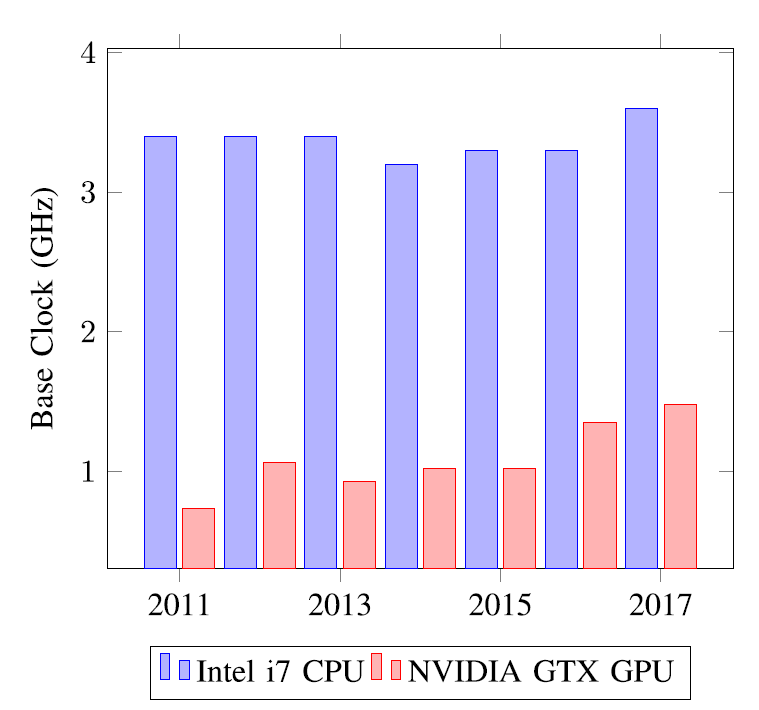
\includegraphics[width=0.6\textwidth]{comparativeCPU_GPU.png}
 \caption{Base clock frequencies of Intel i7 CPU vs. NVIDIA GTX CPU since 2011.
          \label{comparative}}
\end{figure}

Having said that, the GPUs purposes have increased in the late decades, as they
allow that parallel computation (training artificial neural networks and running
optimization algorithms).

Therefore, CPUs are used when the calculations cannot be run in parallel, as
they have superior clock frequencies and more low level memory cache (single
threaded sequential performance) \hyperref[comparative]{\ref{comparative}}.

Actually, five of the top hundred supercomputers have already implemented some
for of heterogeneous computing \cite{cashmere}. 

\section{Dataflow graphs}

A computational graph, other name given to a dataflow graph, is a directed graph
where the nodes describe operations and edges represent data flowing between
these operations. Each of those nodes count with zero or more inputs and zero or
more outputs for the values to flow between nodes (which are represented by
tensors - arrays with arbitrary dimensionality).

TensorFlow actually supports a distributed implementation where client and
processes are run in entirely different machines.

Furthermore, in TensorFlow all data is represented by tensors, independently of
their size or complexity. After having the constructed the graph depending on
the data and functions used, the simulation is run by a greedy heuristic
algorithm.

\section{Particle Swarm Optimization}

\subsection{The classical PSO Algorithm}

The PSO algorithm (Particle Swarm Optimization) is an evolutionary algorithm 
which includes global and local search mechanisms. It simulates a swarm of
particles \cite{particleswarm}. Each volume-less particle occupies a point in the domain of the cost
function  as a set of parameters with length \emph{n}. The amount of particles
\emph{m} is usually chosen based on the scale or complexity of the cost function
\cite{artgpo}.

\begin{equation}
P = [x_{i,j} \in R^{m \times n} | x_{i,j} \sim U([l_{min}, l_{max}])]
\end{equation}

As this is a summary of the main article, it is not going to be specified more
equations used in the PSO algorithm. For more information please reference
article \cite{artgpo}.

\subsection{Modifications and Variants}

PSO has suffered along the years several meta-optimizations. In the variant used
in the summarized paper the previous velocity in the velocity calculation is
scaled by an inertia value $\omega$.

\begin{equation}
v_i := \omega v_i + \varphi_1 s_1(\vec{b_i} - \vec{p_i}) 
    + \varphi_2 s_2(\vec{g} - \vec{p_i})
\end{equation}

Therefore, linearly decreasing inertia values tend to increase performance of
the global and local searches. This leads to a problem, which is that the 
algorithm does not perform well the it has not been restricted by local 
information.

It was found that combining PSO and genetic algorithms leads to better results
than those algorithms separately.

\subsection{Cognitive limitations}

Basically, the algorithm has problems while operating in high dimensions
functions.

\subsection{Transition from PSO to GPO}

The main difference between these algorithms will be found of the way the local
and global search mechanisms interact with one another. In GPO, the local search
is going to be affected by the gradient operator. 

The constant interaction from the global search providing information to the
local search gives the algorithm the ability to coordinate both explorations.

\section{The gradient population optimization algorithm}

The GPO algorithm seeks to exploit the advantage of the GD search for the local
mechanism; and the advantage of the PSO for the global mechanism.

\subsection{GPO algorithm: the fundamental formulation}

The GPO algorithm uses the following formula:

\begin{equation}
P := \omega P + F_l(P) + F_h(P)
\end{equation}

In the previous formula, $\omega P$ represents the inertia factor; while $F_g$
and $F_l$ represents the global and local update factors. The GPO algorithm
leaves $F_g$ unchanged, while rewrites $F_l$.

As for the gradient matrix, it is produced via

\begin{equation}
G = \nabla f(P)
\label{gradientMatrix}
\end{equation}

Where each row of $G$ is the first order derivative of the corresponding
position in the vector in $P$:

\begin{equation}
G{ij} = \frac{\partial f (x_i)}{\partial x_j}, 
i = 1, 2, \ldots, m; 
j= 1, 2, \ldots, n
\label{tensorflowEquation}
\end{equation}

In TensorFlow the gradient expression 
\hyperref[tensorflowEquation]{\ref{tensorflowEquation}} is computed using
special highly-efficient symbolic/numeric routine that makes extensive use of
the graph-like structure of the dataflow implementation of the algorithm.

According to the authors, the formula
\hyperref[gradientMatrix]{\ref{gradientMatrix}} cannot be applied in practice.
The gradient needs to be controlled in order to avoid the algorithm to explode
while updating the evolution.

To do so, authors performed a \emph{two-step clipping procedure}.

\begin{enumerate}
 \item $G$ is clipped by its direct global norm.

  \begin{equation}
  \|G\|_F_r = (\sum_{i=1}^m \sum_{j=1}^n |G_{i,j}|^2)^\frac{1}{2}
  \end{equation}

  Next, the Frobenius norm $\|G\|_F_r$ is used to determine the following scaling
  factor

  \begin{equation}
  \alpha = \frac{\gamma}{max(\|G\|_F_r, \gamma)}
  \label{alphaFactor}
  \end{equation}

  After some experimentation, $\gamma = 2.5$ was the selected value for 
  \hyperref[alphaFactor]{\ref{alphaFactor}} equation.

  Finally, the $\alpha$-factor is applied to the matrix $G$ through the scalar
  multiplication:

  \begin{equation}
  G' = G \alpha
  \end{equation}

 \item Afterwards, $G'$ is coupled with $F_g$ obtaining $G' - F_g$. What it does
 it to clip the first factor by the global optimization best matrix (which is
 the second factor) only if the next condition is fulfilled:
  
  \begin{equation}
  |F_g_{i,j}| < |G'_{i,j}|
  \end{equation}

  The final update is carried by:
  
  \begin{equation}
  F_l = \varphi_l [x_{i,j} \in G' | x_{i,j} = min(|G'_{i,j}|, |F_g_{i,j}|)].
  \end{equation}
\end{enumerate}

According to the authors \textit{This keeps the local factor in check and on
par, in terms of scale, with the relatively tame global factor and makes the use
of gradients in non-convex optimization more stable} \cite{artgpo}.

\section{Metrics}

To assure clearly in the measurement taken in each algorithm, the samples were
taken every 25 epochs. Each result was explained taking into account the result
of each algorithm comparatively and explaining the configuration used to obtain
that solution (as this is a summary of the original article, there will be no
such detail in the explanations given, for more detail please read the whole
article \cite{artgpo}).

In the comparisons, the first tier was made with bi-dimensional functions,
the three remaining tiers where multi-dimensional functions.

Each multidimensional function was separated into ranges:

\begin{enumerate}
 \item $10D, 20D and 30D$ being low-dimension.
 \item $100D, 500D, 10^3D$ comprising medium-dimension.
 \item $10^4D, 10^5D$ for high-dimension functions.
\end{enumerate}

\subsection{Experiment settings}

As part of the experiment, it was used a high-performance computer with the
specifications:

\begin{description}[align=left]
 \item [CPU] Intel i7 5820K with the factory-set clock speed of 3.3GHz.
 \item [GPU] NVIDIA Titan X Pascal with 3584 cores and the factory-set clock
 speed of 1.5GHz.
 \item [RAM] 64GB. 
\end{description}

\begin{table}[h!]
 \centering
  \begin{tabular}
        { | p{0.7cm} | p{3cm} | p{3cm} | p{2cm} | }
  \hline
  Cf. & GPO params. & PSO params. & GD params. \\
  \hline
  $C_1$ & $\varphi_l = 3, \varphi_g = 2$ & $\varphi_1 = 3, \varphi_2 = 2$ &
  \alpha = 0.1 \\
  \hline
  $C_2$ & $\varphi_l, \varphi_g = 2$ & $\varphi_1, \varphi_2 = 2$ & 
  \alpha = 0.01 \\
  \hline
  $C_2$ & $\varphi_l = 2, \varphi_g = 3$ & $\varphi_1 = 2, \varphi_2 = 3$ &
  \alpha = 0.001 \\
  \hline
  \end{tabular}
\caption{Hyper-parameter configurations used for experimentation.}
\end{table}

\section{Results}

The results of the different functions are going to be explained without getting
into much detail, as the objective of this article is to summarize the original
\cite{artgpo}, not to repeat it.

\subsection{Two-dimension function results}

The GPO and PSO algorithms had no problem with these functions. Even though, PSO
needed more iterations than GPO to find the optimum.

\subsection{Low-dimension function results}

\subsubsection{Sphere function in 10, 20 and 30 dimensions}

All of the algorithms were able to find the result.

\subsubsection{Griewank function in 10, 20 and 30 dimensions}

No algorithm found a solution, although GPO and PSO were able to find an
approximation. In general, PSO found obtained the best performance.

\subsubsection{Rastrigin function in 10, 20 and 30 dimensions}

No algorithm found the global optimum. Even though, GPO had the lowest result
average, while PSO had the highest. GD was not able to converge on acceptable
local optima.

\subsubsection{Styblinski-Tang function 10, 20 and 30 dimensions}

No algorithm was able to converge on the global optimum. GPO outperformed PSO
and GD.

\subsection{Mediom-dimension functions}

\subsubsection{Sphere function in 100, 500 ns $10^3$ dimensions}

GPO and GD were able to find the global optimum in every configuration. GPO and
GD obtained better overall performance than PSO.

\subsubsection{Griewank function in 100, 500 and $10^3$ dimensions}

No algorithm was able to find the global optimum. GPO was the one which
approximated the most (asymptotically).

\subsubsection{Rastrigin function in 100, 500 and $10^3$ dimensions}

GPO found the best result in 100D. On average, PSO had the highest result. GD
did not provide an acceptable result.

\subsubsection{Rosenbrock function in 100, 500 and $10^3$ dimensions}

GPO was the only algorithm that found the global optimum. PSO gave acceptable
results, but had a higher result on average. GD was not able to produce
acceptable results.

\subsubsection{Styblinski-Tang function in 100, 500 and $10^3$ dimensions}

No algorithm was able to find the global optimum. However, GD achieved better
result int 500D and $10^3D$.

\subsection{High-dimension functions}

\subsubsection{Sphere function in $10^4$ and $10^5$ dimensions}

GPO and GD were able to find the global optimum. PSO was not able to converge in
the global optimum in any of the samples.

\subsubsection{Rastrigin function in $10^4$ and $10^5$ dimensions}

No algorithm was able to approximate the global optimum. GD obtained the best
results.

\subsubsection{Rosenbrock function in $10^4$ and $10^5$ dimensions}

GPO provided the best results. PSO achieved acceptable results. GD was not able
to provide satisfactory results.

\subsubsection{Styblinski-Tang function in $10^4$ and $10^5$ dimensions}

Both GD and GPO provided acceptable results. PSO could not ameliorate past the
initialization range.

\subsection{Algorithm scalability}

In general, the PSO algorithm found scalability difficulties as the dimensions
increased. On the other hand, GPO did not find problems in great deal of the
functions (only has problems with Rastrigin function). Finally, GD, which had no
problem in the Sphere and in the Styblinski-Tang functions, but found lots of
problems in the rest of the functions.

\subsection{Runtime}

\subsubsection{PSO NumPy and TensorFlow CPU variants}

Summarized in the graph \hyperref[runtimeCpu]{\ref{runtimeCpu}}.

\begin{figure}[h!]
 \centering
 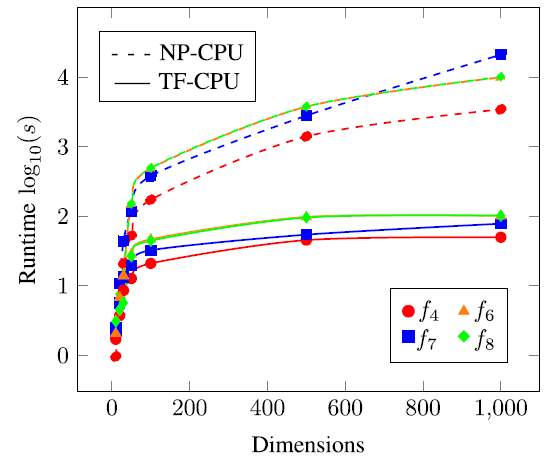
\includegraphics[width=0.6\textwidth]{runtimeCpu.png}
 \caption{Runtime of PSO variants NP-CPU and TF-CPU on multi-dimension samples.
          \label{runtimeCpu}}
\end{figure}

\subsubsection{PSO TensorFlow CPU and GPU variants}

Summarized in the graph \hyperref[runtimeCpuGpu]{\ref{runtimeCpuGpu}}.

\begin{figure}[h!]
 \centering
 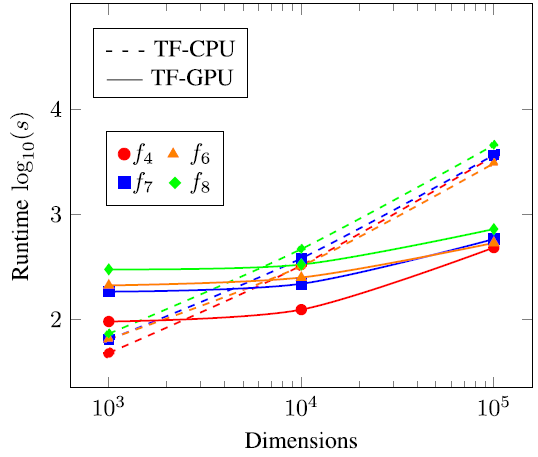
\includegraphics[width=0.6\textwidth]{runtimeCpuGpu.png}
 \caption{Runtime of PSO variants TF-CPU and TF-GPU on multi-dimension samples.
          \label{runtimeCpuGpu}}
\end{figure}

\subsubsection{GPO and PSO TensorFlow GPU variants}

Summarized in the graph \hyperref[runtimeGpu]{\ref{runtimeGpu}}.

\begin{figure}[h!]
 \centering
 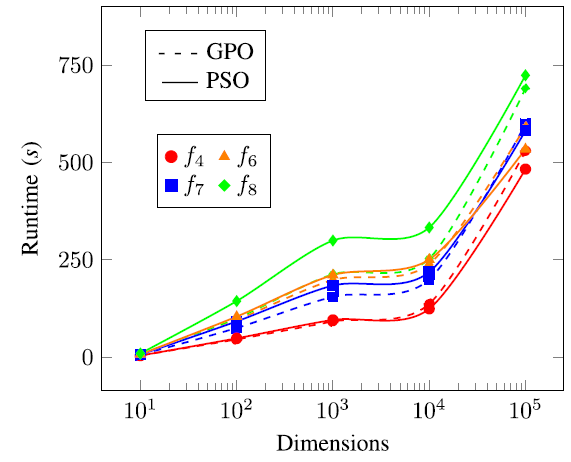
\includegraphics[width=0.6\textwidth]{runtimeGpu.png}
 \caption{Runtime of GPO and PSO using TF-GPU variants.
          \label{runtimeGpu}}
\end{figure}

\section{Conclusion}

According to the authors, the integration of the gradient into the local search
mechanism was a success, allowing small populations to optimize exceptionally
large problems. Although large populations may cause an increased runtime, or
intractable optimization problems.

Overall, GPO obtained good results on most of the tested functions regardless
the dimensionality (with less iterations than PSO).

\section*{Bibliography}

\printbibliography

\end{document}
